\subsection{Advection stabilisation}\label{sec:advection}
The 1D advection problem proposed by \citet{Donea2003} and \citet{Thieulot2011} is performed to verify the effectiveness of the SUPG method to stabilise the
advection term of the energy equation. The domain is a 1D segment with $L_x=1$ composed by 50 elements and a discontinuity in the thermal field placed at
$x=0.25$. Temperature is set to 1 for $x \leq 0.25$ and to 0 for $x > 0.25$. Velocity is set to ${u}=1$ in the entire domain. The simulation is performed for
250 time steps, with $dt=0.002$, so the thermal discontinuity should be at $x=0.75$ at the end of the simulation.

Temperature profiles at the end of the simulation are shown in Fig. \ref{fig:advection} as function of the dimensionless coefficient $\gamma=\tau \bm{v}/h$. In case
of the classic Galerkin method ($\gamma=0$, blue line in Fig. \ref{fig:advection}) the final thermal profile is characterised by strong oscillations, which are
eliminated in case of the SUPG method ($\gamma=0.045$, orange line in Fig. \ref{fig:advection}).
All data can be found at \url{https://github.com/aleregorda/Benchmarks/tree/main/Energy_equation/Advection_stabilisation}.

\begin{figure}[h!]
\centering
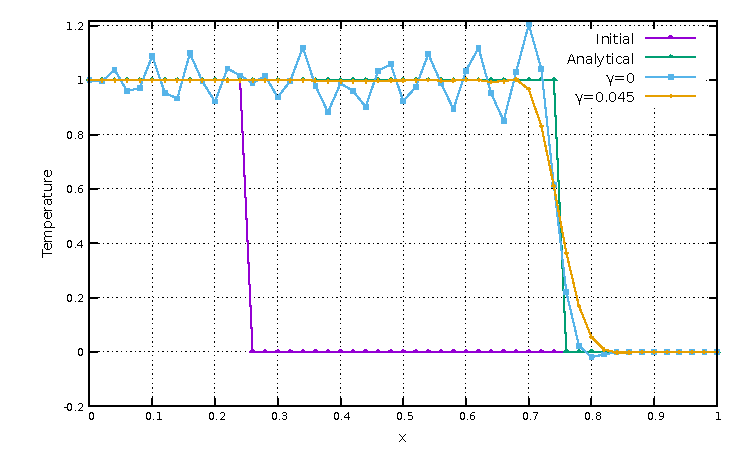
\includegraphics[width=9.5cm]{./Figures/Advection.pdf}
\caption{Temperature profile as function of \textit{x} for the advection stabilisation benchmark. Purple line indicates the initial temperature profile; the
green line indicates the analytical temperature profile after 250 time steps; blue line indicates the temperature profile after 250 time steps in case of the
classic Galerkin method ($\gamma=0$); orange line indicates the temperature profile after 250 time steps in case of the SUPG method ($\gamma=0.045$).}
\label{fig:advection}
\end{figure}
